\chapter{数据的处理与导入}
	\chaptermark{数据的处理与导入}
	\section{系统要求}
	Web端基因组浏览器对于GFF数据支持的比较完善,对于数据的处理方式相同,但由于GFF数据格式存在的版本的差异性,同时GBrowse及其它基因组浏览器对于GFF3的支持最为完善,并逐步在废弃低版本的GFF格式数据,本小节以GBrowse为例说明对GFF3数据处理的方式。
	\subsection{GFF3数据格式}
	GFF格式是Sanger研究所定义,是一种简单的、通用的、方便的对DNA、RNA以及蛋白质序列的特征进行描述的一种数据格式,比如序列的那里到那里是基因,已经成为序列注释的通用格式,比如基因组的基因预测。GFF格式比较主流的有两个版本GFF2和GFF3,其都以纯文本文件进行存储数据,都包含9列,使用制表符分隔文件。但GFF3在GFF2的基础上进行了修改和增强,对于部分列信息进行修改,解决了GFF2只能表现一个层次的嵌套功能及没有层次结构方向的任何概念等一些列问题。\\
	\indent 在GFF3格式的数据中,每一列具体的含义见表4.1。attributes列以多个键值对组成的注释信息描述,键与值之间用“=”,不同的键值用“:”隔开,一个键可以有多个值,不同值用“,”分割。注意如果描述中包括Tab键以及“,=;”,要用URL转义规则进行转义,如Tab键用 “\%09”代替。键是区分大小写的,以大写字母开头的键是预先定义好的,在后面可能被其他注释信息所调用。具体名称及含义见表4.2。
	\begin{table}[!htbp]
		\centering
		\begin{tabular}{ll}	
			\toprule
			列名称& 含义\\
			\midrule
			seqid&文档信息及示例\\
			source&source是文本限定符,旨在描述生成此功能的算法或操作过程\\
			type&功能的类型\\
			start&特征的开始 \\
			end&特征的结束\\
			strand&特征链,+为正链(相对于地标), - 为负链\\
			phase&CDS类型的功能描述区域\\
			attributes&以多个键值对组成的注释信息描述\\
			\bottomrule
		\end{tabular}
		\caption{GFF3数据格式及含义}
	\end{table}
	
	\begin{table}[!htbp]
		\centering
		\begin{tabular}{ll}	
			\toprule
			列名称& 含义\\
			\midrule
			ID&文档信息及示例\\
			Name&显示该功能的名称\\
			Alias&显示该功能的名称\\
			Parent&表示功能的父级 \\
			Target&表示核苷酸对核苷酸或蛋白质至核苷酸比对的靶标\\
			Gap&如果两者不共线,则该特征与目标的对齐(例如,包含间隙)\\
			Derives\_from&用于消除一个特征与另一个特征之间的关系\\
			Note&对基因信息的描述\\
			Dbxref&数据库交叉引用\\
			Ontology\_term&对本体术语的交叉引用\\
			Is\_circular&标识是否为圆形\\
			\bottomrule
		\end{tabular}
		\caption{属性名称及含义}
	\end{table}
	\section{数据转储}
	GBrowse不是直接访问GFF格式,而是需要全部载入内存,或者导入数据库中,成为更为结构化的、或者模式数据,以统一的数据库访问接口,供GBrowse调用数据。如表4.3,GBrowse中对数据接口的支持。在GBrowse中默认加载GFF3数据的默式是从内存中读取数据,由于基因组数据实际很大,不适合直接存储到内存中,因此选用MySQL关系型数据库进行数据存储。
	\begin{table}[!htbp]
		\centering
		\begin{tabular}{ll}	
			\toprule
			列名称& 含义\\
			\midrule
			Bio::DB::SeqFeature::Store&GFF3格式支持的GBrowse官方推荐的数据库\\
			Bio::DB::Das::Chado&GMOD支撑的通用的生物信息学数据库模式\\
			Bio::Das&分布式注释系统\\
			Bio::DB::Das::BioSQL&一个通用的生物信息学数据库模式 \\
			Bio::DB::GFF&基于GFF2的数据库系统 \\
			\bottomrule
		\end{tabular}
		\caption{GBrowse数据库接口}
	\end{table}
	\subsection{数据库表结构}
	\begin{figure}
		\centering
		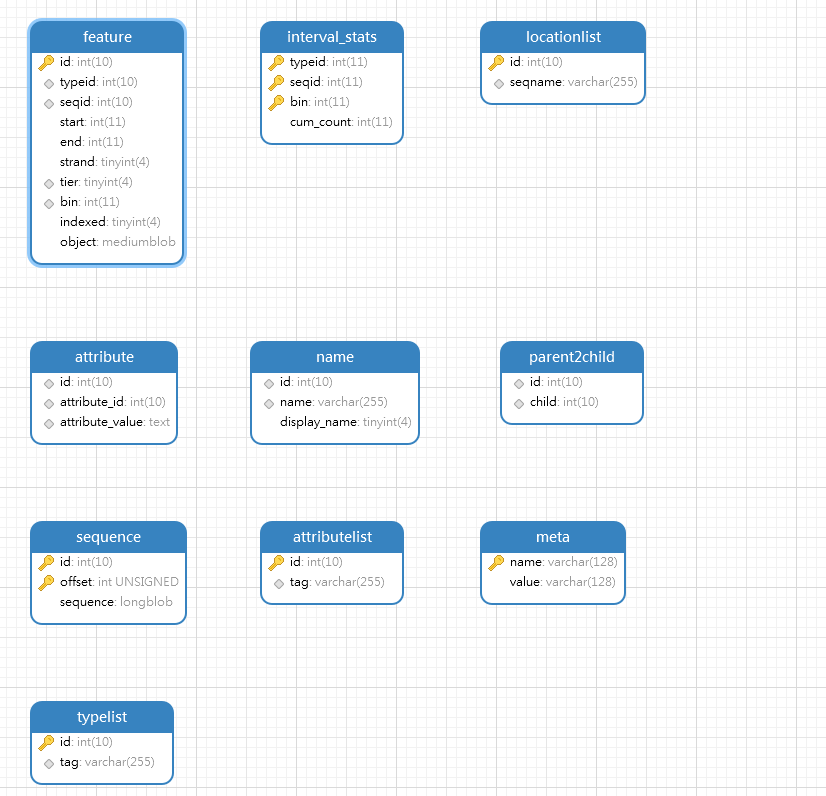
\includegraphics[width = .6\textwidth]{4-1.png}
		\caption{GBrowse页面内容展示图}
	\end{figure}
	\subsection{转储操作}
	在转储苹果基因组操作中,首先创建苹果基因数据库malus,其次通过使用GBrowse中提供bp\_seqfeature\_load脚本工具创建和录入GFF3数据到MySQL数据中。需要对脚本相关选项参数进行配置。参数详情见表4.4。最后通过配置数据库权限,使服务器能读取数据。详细处理代码如下。\\
	\begin{lstlisting}[language=bash]
	mysql -uroot -proot
	create database malus
	/usr/bin/bp_seqfeature_load -a DBI::mysql -d malus -u root \
	-p root --create malus.gff3
	mysql -uroot -p password -e \
	'grant all privileges on genomegff3.* to me@localhost'
	mysql -uroot -p password -e \
	'grant select on genomegff3.* to apache@localhost'
	\end{lstlisting}
	\begin{table}[!htbp]
		\centering
		\begin{tabular}{ll}	
			\toprule
			列名称& 含义\\
			\midrule
			-d --dsn&数据连接信息\\
			-s --seqfeature&序列特征类型\\
			-a --adaptor&存储适配器类型\\
			-f --fast&激活快速转储 \\
			-c --create&需转换的GFF3数据源 \\
			-u --user&数据库连接用户 \\
			-p --password&数据库连接密码 \\
			\bottomrule
		\end{tabular}
		\caption{脚本选项参数}
	\end{table}
	\subsection{数据源配置文件编写}
	在苹果基因组数据配置文件malus.conf文件中,指明该数据源访问接口,已经主机、用户名等访问参数。具体操作代码如下。
	\begin{lstlisting}[language=bash]
	[GENERAL]
	database	= chromosomes
	[alternative:database]
	db_adaptor    = Bio::DB::SeqFeature::Store
	db_args       = -adaptor DBI::mysql
	-dsn    dbi:mysql:database=malus_alternative;host=localhost
	-user   root
	-pass   root
	\end{lstlisting}